In Figure \ref{fig:network_biology_evolution} we can see a representation of the evolution for visualization of networks in system biology. Before the computers, networks were represented in 2 dimensions and they were static representations that lacked interactivity, see Figure \ref{fig:network_biology_evolution} A. With the computer era and the advancement in computer graphics, 3D representations were possible, with the addition of interactions (See Figure  \ref{fig:network_biology_evolution} C). As computer science progressed, visualization improved and also new technologies emerged like virtual reality, which has a huge potential with regards to the interactivity (Figure \ref{fig:network_biology_evolution} I).

\begin{figure}[h!]
    \newlength{\tempheight}
    \setlength{\tempheight}{15ex}
    \centering%
    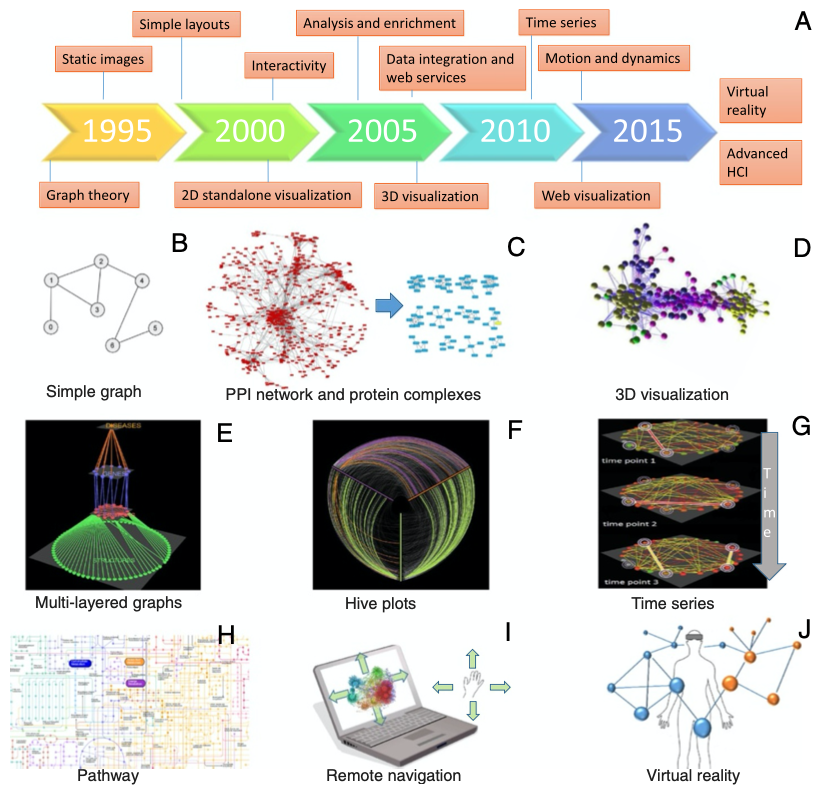
\includegraphics[width=\textwidth]{evolution_visualization}
    \caption{Visualization for network biology. a Undirected unweighted graph showing co-expression relationship between genes. b A 2D representation of a yeast protein-protein interaction network visualized in Cytoscape (left) and potential protein complexes 3D identified by the MCL algorithm from that network (right). c A 3D network of genes showing co-expression relationships. d A multilayered network integrating different types of data visualized by Arena3D. e A hive plot view of a network where nodes are mapped to and positioned on radially distributed linear axes. f Visualization of network changes over time. g Static picture showing part of lung cancer pathway. h Navigation of networks using hand gestures. i Integration and control of 3D networks using VR devices. Figure adapted\cite{pavlopoulos_malliarakis_papanikolaou_theodosiou_enright_iliopoulos_2015}.}
    \label{fig:network_biology_evolution}
\end{figure}
